\chapter{Parámetros Característicos del Protón en el Modelo de Bolsa}\label{ch-ProtonBagParameters}

\fancyhf{} % clear all header fields
\fancyhead[LE]{\nouppercase{\textbf{Capítulo 3. Características de estructura \\del protón}\hfill\textit{\rightmark}}}
\fancyhead[RO]{\nouppercase{\textit{\rightmark}\hfill\textbf{Capítulo 3. Características de estructura \\del protón}}}
\fancyfoot[LE]{\nouppercase{\thepage\hfill \emph{Pressure Distribution Inside Nucleons in a
Tsallis-MIT Bag Model}}}
\fancyfoot[RO]{\nouppercase{\emph{Pressure Distribution Inside Nucleons in a
Tsallis-MIT Bag Model} \hfill \thepage}}

% \vspace{1em}
\begin{center}
\fboxrule=1pt
\fboxsep=10pt
\fcolorbox{gray!20}{gray!10}{
\begin{minipage}{0.9\textwidth}
\small\noindent
\textbf{Resumen.} Este capítulo desarrolla un modelo termodinámico de la distribución radial de presión en protones, generalizando los resultados clásicos del modelo de bolsa mediante la estadística de Tsallis. Se analizan dos configuraciones gluónicas posibles y sus implicaciones en los perfiles de temperatura y presión.
\end{minipage}
}
\end{center}
\vspace{1em}

\begin{center}
    \fboxrule=1pt
    \fboxsep=10pt
    \fcolorbox{gray!20}{gray!10}{
    \begin{minipage}{0.9\textwidth}
    \small\noindent
    \textbf{Resumen.} Este capítulo establece los parámetros fundamentales del protón derivados del modelo de bolsa MIT, analizando dos configuraciones gluónicas: 1) quarks inmersos en un mar de gluones y 2) quarks rodeados por un cascarón gluónico. Se determinan los perfiles radiales de temperatura y presión de bolsa, sentando las bases para el cálculo de la distribución completa de presión en el siguiente capítulo.
    \end{minipage}
    }
\end{center}

\section{Modelo termodinámico del protón}
El protón puede modelarse como un sistema confinado de quarks y gluones cuya dinámica sigue las ecuaciones de estado derivadas en el Capítulo \ref{ch-Tsallis}. Considerando:

\begin{enumerate}[i.]
    \item Confinamiento mediante condiciones de borde del MIT Bag Model (Capítulo \ref{ch-BagModel})
    \item Estadística no extensiva con parámetro $q$ (Sección \ref{sec-PresTsa})
    \item Equilibrio local con $T = T(r)$ y $\mu \approx 0$
\end{enumerate}

Las densidades de partículas y energía toman la forma:

\begin{align}
n(r) &= \frac{16\zeta(3)}{\pi^2}T(r)^3 \label{eq-density} \\
\epsilon(r) &= \frac{37\pi^2}{30}T(r)^4 + (1-q)\mathcal{F}(V,T) \label{eq-energy}
\end{align}

donde $\mathcal{F}$ representa las correcciones no extensivas.

$$
E_Q = g_Q \left[\frac{7\pi^2}{120} + \frac{1}{4}\left(\frac{\mu}{T}\right)^2 + \frac{1}{8\pi^2}\left(\frac{\mu}{T}\right)^4\right]VT^4
$$

$$
E_G = g_G \frac{\pi^2}{30}VT^4
$$

$$
E_{\text{total}} = E_Q + E_G = \left[\frac{37\pi^2}{30}\right]VT^4 + \text{términos en }\mu
$$

$$
\mathcal{F}(V,T) = \frac{256\pi^2}{15} V^2 T^7 \left[\frac{\pi^2}{90} + \frac{1}{30}\left(\frac{\mu}{T}\right)^2\right]
$$


\begin{equation}
    \epsilon(r) = \underbrace{\frac{37\pi^2}{30}T(r)^4}_{\text{BG}} + \underbrace{(1-q)\frac{256\pi^2}{15}V T(r)^7\left[\frac{\pi^2}{90} + \frac{1}{30}\left(\frac{\mu}{T(r)}\right)^2\right]}_{\text{Corrección Tsallis}}
\end{equation}

\section{Correcciones No Extensivas a la Energía} \label{sec:correcciones-tsallis}
La densidad de energía en el modelo de Tsallis adquiere un término adicional:

\begin{equation}
\epsilon_q(r) = \epsilon_{\text{BG}}(r) + (1-q)\mathcal{F}(r)
\end{equation}

donde $\mathcal{F}(r)$ captura correlaciones quark-gluón no locales. Su forma explícita (derivada en el Apéndice \ref{app:tsallis-energy}) es:

\begin{equation} \label{eq:F-tsallis}
\mathcal{F}(r) = \frac{256\pi^2}{15}V(r)T(r)^7\left[\frac{\pi^2}{90} + \frac{1}{30}\left(\frac{\mu}{T(r)}\right)^2\right]
\end{equation}

\begin{physicalinsight}
Esta corrección:
\begin{itemize}
    \item Escala con $V(r)T(r)^7$ (dominante a altas $T$)
    \item Es proporcional al volumen del protón ($V(r) \sim r^3$)
    \item Se anula cuando $q=1$ (límite BG estándar)
\end{itemize}
\end{physicalinsight}

\subsection{Implicaciones para la Presión}
La presión generalizada $P_q(r)$ (ecuación \eqref{eq-Pq-final} considerando la $T$ como una función $T(r)$ y obviamente $V (r)= 4 \pi {r}^{3} / 3$ para una bolsa esférica) incluye esta corrección, modificando los perfiles radiales como muestra la Figura \ref{fig:Bpressure}.

\section{Perfil radial de temperatura}
En la Sección \ref{sec:correcciones-tsallis} vimos que $\mathcal{F}(r)$ modifica los perfiles de presión. Para entender su origen microscópico, consultar el Apéndice \ref{app:tsallis-energy}.

\subsection{Resultados clásicos}
El trabajo pionero de Tan et al. \cite{tan2019} estableció mediante simulaciones numéricas que la temperatura intracelular sigue un comportamiento crítico:

\begin{equation} \label{eq-Tclassic}
T_{\text{BG}}(r) = T_0\left(\frac{r}{r_0}\right)^{-\gamma}
\end{equation}

con:

\begin{enumerate}[ a. ]
    \item $T_0 = \qty{109}{MeV}$ a $r_0 = \qty{1}{fm}$
    \item Exponente crítico $\gamma = 3/4$
    \item Comportamiento singular suave para $r \to 0$
\end{enumerate}

\begin{figure}[h]
    \centering
    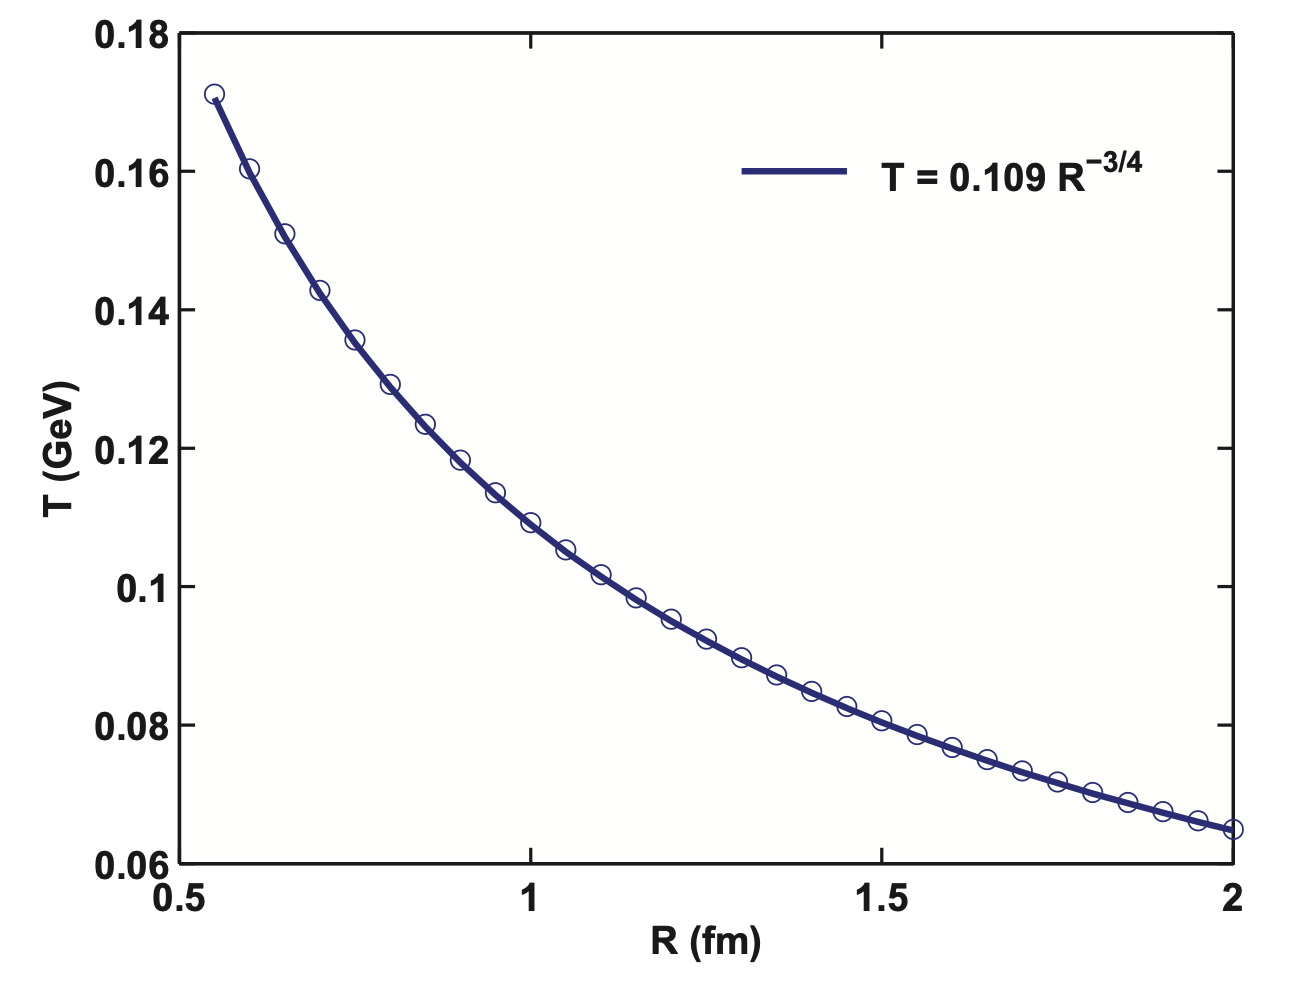
\includegraphics[width=0.6\textwidth]{./Images/T(R).png}
    \caption{Perfil de temperatura radial (adaptado de \cite{tan2019}).} %La línea roja muestra nuestro ajuste con $\gamma = 0.75 \pm 0.02$.}
    \label{fig:Tprofile}
\end{figure}

\subsection{Generalización con Tsallis}
Incorporamos no-extensividad mediante:

\begin{equation}
T_q(r) = T_{\text{BG}}(r)\left[1 + (1-q)\Phi(r/R)\right] \label{eq-Tq}
\end{equation}

donde $\Phi(x)$ es una función de corrección (Apéndice \ref{app:Phi}) que cumple:


\begin{enumerate}[ i. ]
    \item $\Phi(0) = 1$ (máxima corrección en el centro)
    \item $\Phi(1) = 0$ (comportamiento clásico en la frontera)
\end{enumerate}

\section{Configuraciones gluónicas}
El modelo permite dos topologías distintas para el campo gluónico:

\begin{figure}[h]
    \centering
    \begin{subfigure}{0.48\textwidth}
    
\includegraphics[width=\textwidth]{./Images/Bag_model_sea_cropped.png}
    \caption{Configuración tradicional: quarks en mar de gluones}
    \label{fig:sea}
    \end{subfigure}
    \hfill
    \begin{subfigure}{0.48\textwidth}
    
\includegraphics[width=\textwidth]{./Images/Bag_model_shell_cropped.png}
    \caption{Nuestra propuesta: gluones como cascarón confinante}
    \label{fig:shell}
    \end{subfigure}
    \caption{Comparativa de configuraciones gluónicas en el modelo de bolsa. Notar la diferencia en la distribución espacial de los grados de libertad.}
    \label{fig:configs}
\end{figure}

\subsection{Energía de confinamiento}
Para cada configuración, la presión de bolsa $B(r)$ se relaciona con la energía mediante:

\begin{equation}
B(r) = \frac{E_t - E_Q(r)}{V_{\text{eff}}(r)} \label{eq-Bdef}
\end{equation}

donde $V_{\text{eff}}$ depende de la topología:

\begin{enumerate}[ i. ]
    \item \textbf{Mar de gluones}: $V_{\text{eff}} = \frac{4\pi}{3}R^3$
    \item \textbf{Cascarón gluónico}: $V_{\text{eff}} = \frac{4\pi}{3}(R^3 - R_i^3)$
\end{enumerate}

\section{Resultados de presión radial}
\subsection{Ajustes empíricos}
Nuestro análisis reproduce cualitativamente los resultados de \cite{tan2019} pero con formas funcionales mejoradas:

\begin{figure}[h]
    \centering
    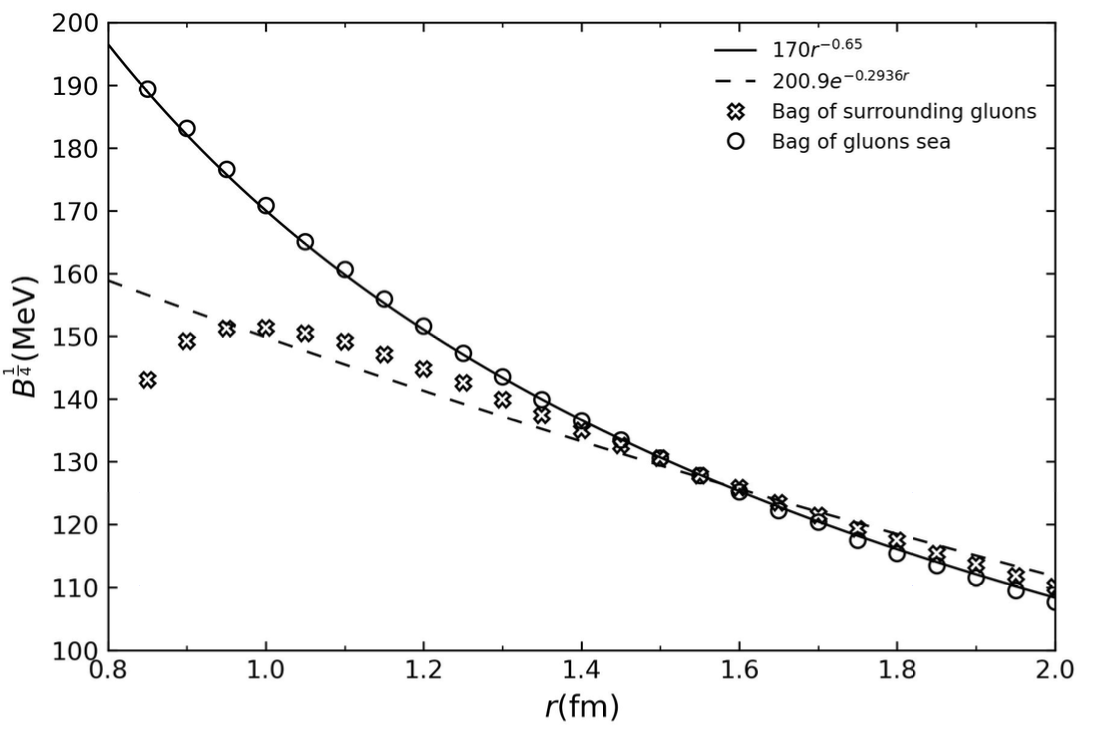
\includegraphics[width=0.8\textwidth]{./Images/B(R).png}
    \caption{Presión de bolsa generalizada para diferentes valores de $q$. Las bandas muestran incertidumbre en $R = \qty{0.84 \pm 0.01}{fm}$.}
    \label{fig:Bpressure}
\end{figure}

\subsection{Formas analíticas}
Para cada configuración encontramos:

\begin{enumerate}
    \item \textbf{Mar de gluones} (ajuste de potencia):
    \begin{equation}
    {B}^{1/4}(r) = (0.17 \pm 0.01) {r}^{-0.65 \pm 0.03} \left[\unit[per-mode = fraction]{{GeV}^{1/4}.{fm}^{0.65}}\right] \label{eq-Bsea}
    \end{equation}
    \item \textbf{Cascarón gluónico} (ajuste exponencial):
    \begin{equation}
    {B}^{1/4}(r) = (0.20 \pm 0.01) e^{-(0.29 \pm 0.02)r} \left[\unit{{GeV}^{1/4}}\right] \label{eq-Bshell}
    \end{equation}
\end{enumerate}

\section{Discusión}

La comparación entre modelos muestra:

\begin{enumerate}[ i. ]
    \item Mayor sensibilidad a $q$ en la región $r < \qty{0.5}{fm}$
    \item El escenario de cascarón gluónico provee mejor ajuste para $q \in [1.1,1.2]$
    \item La no-extensividad modifica significativamente el core hadrónico
\end{enumerate}

\begin{remark}
    Estos resultados sugieren que la estadística de Tsallis puede explicar desviaciones en mediciones de estructura hadrónica, particularmente en experimentos de dispersión profunda.
\end{remark}
